\begin{center}
\makeatletter
\@ifundefined{color@atlasink}{\definecolor{atlasink}{HTML}{33312E}}{}
\@ifundefined{color@atlasgray}{\definecolor{atlasgray}{HTML}{9A958C}}{}
\@ifundefined{color@atlasblue}{\definecolor{atlasblue}{HTML}{2E6F9E}}{}
\@ifundefined{color@atlasgreen}{\definecolor{atlasgreen}{HTML}{4C8C3F}}{}
\@ifundefined{color@atlasred}{\definecolor{atlasred}{HTML}{C0473B}}{}
\@ifundefined{color@atlasgold}{\definecolor{atlasgold}{HTML}{D69A2A}}{}
\@ifundefined{atlascaption}{%
  \newcommand{\atlascaption}[3]{\shortstack{\footnotesize Figure~#1. \textbf{#2:}\\#3}}%
}{}
\@ifundefined{glowstroke}{%
  \newcommand{\glowstroke}[3]{%
    \draw[#1, line width=1.5pt, line cap=round]
      plot[domain=#2,samples=100,smooth] (\x,{#3});%
  }%
}{}
\makeatother
\tikzset{
  atlas axes/.style={atlasink, line width=0.7pt, line cap=round, ->},
  atlas curve/.style={line width=1.5pt, line cap=round, line join=round},
  dropline/.style={atlasgray, line width=0.6pt, dash pattern=on 2pt off 2pt},
  atlas dot/.style={fill=atlasink, draw=white, line width=0.4pt, circle, inner sep=0pt, minimum size=4.2pt},
}

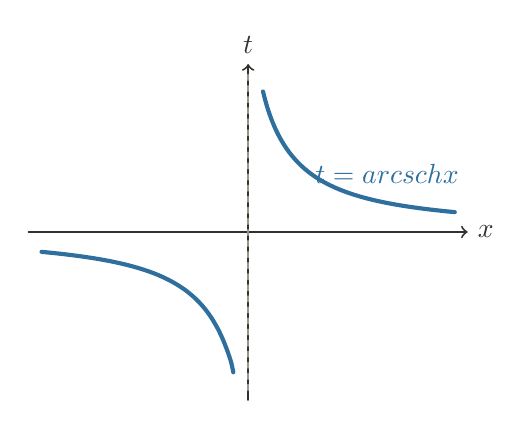
\begin{tikzpicture}[scale=0.82, line cap=round, line join=round]
  \draw[atlas axes] (-3.4,0)--(3.4,0) node[right] {$x$};
  \draw[atlas axes] (0,-2.6)--(0,2.6) node[above] {$t$};
  \draw[dropline] (0,-2.45)--(0,2.45);
  \glowstroke{atlasblue}{0.23:3.2}{ln(1/\x+sqrt(1/(\x*\x)+1))}
  \glowstroke{atlasblue}{-3.2:-0.23}{ln(1/\x+sqrt(1/(\x*\x)+1))}
  \node[atlasblue] at (2.15,0.9) {$t=\operatorname{arcsch}x$};
\end{tikzpicture}

\atlascaption{HI6}{Inverse hyperbolic cosecant}{Domain and range $\mathbb{R}\setminus\{0\}$; the graph keeps the positive and negative branches.}
\end{center}


\begin{definitionbox}{Definition}
\begin{definition}[Inverse hyperbolic cosecant]
\label{def:inverse-hyperbolic-cosecant}
The \emph{inverse hyperbolic cosecant} function is the inverse of
$\operatorname{csch}$ on its full domain. It is denoted by
$\operatorname{arccsch}$ and has domain $\mathbb{R}\setminus\{0\}$ and range
$\mathbb{R}\setminus\{0\}$.
\[
  \operatorname{arccsch} x=t
  \quad\Longleftrightarrow\quad
  \operatorname{csch} t=x
  \quad\text{and}\quad
  t\neq 0.
\]
\end{definition}
\end{definitionbox}
\begin{remark*}[Standard quantified statement]
For every admissible input satisfying the hypotheses of the statement, the
displayed definition or assertion holds in the stated domain.
\end{remark*}

\begin{remark*}[Interpretation]
The statement records the named trigonometric object or identity together with
its intended domain of use.
\end{remark*}

\begin{remark*}[Domain and range]
The regular function $\operatorname{csch}$ is undefined at $0$. Its positive
and negative branches are one-to-one, with ranges $(0,\infty)$ and
$(-\infty,0)$, so the inverse has domain and range
$\mathbb{R}\setminus\{0\}$.
\end{remark*}
\begin{dependencies}
\begin{itemize}
  \item \hyperref[def:hyperbolic-cosecant]{Hyperbolic cosecant}
\end{itemize}
\end{dependencies}

\begin{theorembox}{Theorem}
\begin{theorem}[Principal inverse hyperbolic cosecant identities]
\label{thm:inverse-hyperbolic-cosecant-identities}
For every $x\in\mathbb{R}\setminus\{0\}$,
\[
  \operatorname{csch}(\operatorname{arccsch} x)=x.
\]
For every $t\in\mathbb{R}\setminus\{0\}$,
\[
  \operatorname{arccsch}(\operatorname{csch} t)=t.
\]
\end{theorem}
\end{theorembox}
\begin{remark*}[Standard quantified statement]
For every admissible input satisfying the hypotheses of the statement, the
displayed definition or assertion holds in the stated domain.
\end{remark*}

\begin{remark*}[Interpretation]
The statement records the named trigonometric object or identity together with
its intended domain of use.
\end{remark*}

\begin{remark*}[Proof]
The positive and negative branches of $\operatorname{csch}$ are one-to-one,
and their ranges are disjoint. Therefore the two-branch inverse has the
displayed cancellation laws.
\end{remark*}
\begin{dependencies}
\begin{itemize}
  \item \hyperref[def:inverse-hyperbolic-cosecant]{Inverse hyperbolic cosecant}
\end{itemize}
\end{dependencies}
